% !TeX spellcheck = cs_CZ
{\tikzset{external/prefix={tikz/FYZII/}}
 \tikzset{external/figure name/.add={ch40_}{}}
%---------------------------------------------------------------------------------------------------
% file fey2ch40.tex
%---------------------------------------------------------------------------------------------------
%=========================== Kapitola Proudění "suché vody" ========================================
\chapter{Proudění \uv{suché vody}}\label{fyz:IIchapXL}
\minitoc
  \section{Hydrostatika}\label{fyz:IIchapXLsecI}
    Proudění tekutin a zvláště vody fascinuje každého člověka. Všichni si pamatujeme, jak jsme si v 
    dětství hrávali s touto zvláštní látkou ve vaně nebo v blátivé kaluži. Jak stárneme, pozorujeme 
    potoky, vodopády a víry a jsme okouzleni touto látkou, která v porovnání pevnými látkami vypadá 
    jako živá. Chování tekutin je v mnoha směrech nečekané a zajímavé, a právě to bude tématem této 
    a následující kapitoly. Úsilí dítěte přehradit malý potůček na ulici a jeho překvapení nad tím, 
    jak podivně si voda najde únikovou cestu, mají svou analogii v našich mnohaletých pokusech 
    pochopit proudění kapalin. Snažili jsme se v naší teorii „přehradit vodu“ odvozením zákonů a 
    rovnic, které popisují proudění. Popíšeme takové pokusy v této kapitole. V následující kapitole 
    ukážeme originální způsob, jakým voda prolomila naši hráz a unikla pokusům vysvětlit její 
    chování.
    
    Předpokládáme, že základní vlastnosti vody vám jsou už známé. Hlavní vlastností, která odlišuje 
    tekutinu od pevné látky, je to, že tekutina není schopná ani chvíli udržet smykové napětí. 
    Působíme-li na ni smykovým napětím, dá se do pohybu. Hustější tekutiny, jako med, se pohybují 
    obtížněji než např. vzduch nebo voda. Mírou toho, jak snadno se tekutina poddá napětí je její 
    viskozita. V této kapitole si budeme všímat jen těch situací, v nichž lze vliv viskozity 
    zanedbat. Viskózními jevy se budeme zabývat v následující kapitole.
    
    Nejdříve se budeme věnovat \textbf{hydrostatice}, teorii kapalin v klidu. Jsou-li kapaliny v 
    klidu, neexistují v nich smykové síly (dokonce ani ve viskózních kapalinách). Základní zákon 
    hydrostatiky tedy zní, že napětí jsou vždy kolmá na libovolnou plochu uvnitř kapaliny. Kolmá 
    síla na jednotku plochy se nazývá \textbf{tlak}. Ze skutečnosti, že v klasické kapalině smyky 
    nejsou, vyplývá, že tlakové napětí je stejné ve všech směrech (obr. \ref{fyz_fig544}). Necháme 
    vás, abyste se pobavili důkazem, že nedochází-li na žádné ploše v kapalině ke smyku, musí být 
    tlak stejný v každém směru.
    
    \begin{figure}[ht!] %\ref{fyz_fig544}
      \centering
      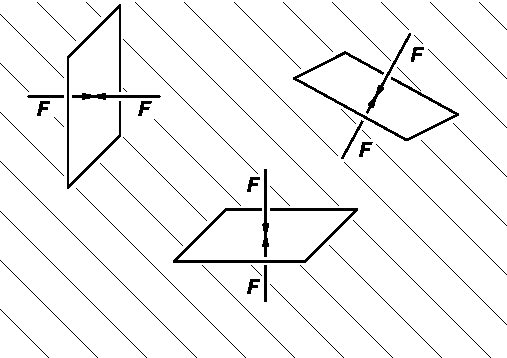
\includegraphics[width=0.7\linewidth]{fyz_fig544.pdf}
      \caption{Ve statické kapalině je síla na jednotku určité plochy kolmá na tuto plochu a má 
               stejnou velikost při libovolné orientaci plochy. 
               (\cite[s.~741]{Feynman02})}
      \label{fyz_fig544}
    \end{figure}

    Tlak v kapalině se může od místa k místu měnit. Například ve statické kapalině na zemském 
    povrchu se tlak mění s výškou, protože působí tíha kapaliny. Považujeme-li hustotu kapaliny 
    \(\varrho\) za konstantní a tlak na nějaké (libovolně zvolené) úrovni je \(p_0\) (obr. 
    \ref{fyz_fig545}) je tlak ve výšce \(h\) nad touto úrovní \(p=p_0 - \varrho gh\), přičemž \(g\) 
    je tíhová síla, která působí na jednotkovou hmotnost. Součet
    \begin{equation*}
      p + \varrho gh
    \end{equation*}
    je proto u statické kapaliny konstantní. Tento vztah je nám znám, ale nyní odvodíme obecnější 
    výsledek, jehož je poslední vztah jen speciálním případem.
    
    \begin{figure}[ht!] %\ref{fyz_fig545}
      \centering
      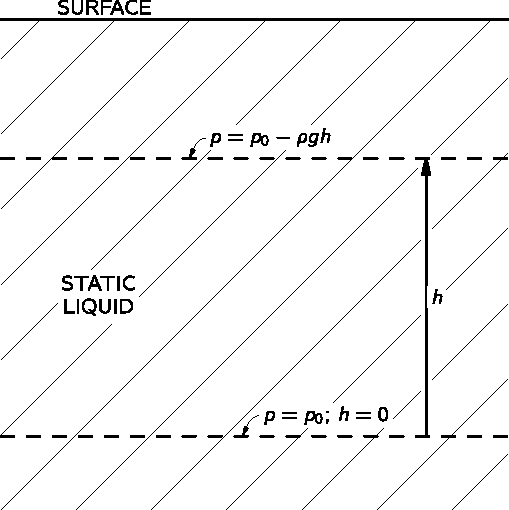
\includegraphics[width=0.7\linewidth]{fyz_fig545.pdf}
      \caption{Tlak ve statické kapalině
               (\cite[s.~741]{Feynman02})}
      \label{fyz_fig545}
    \end{figure}
    
    Představme si malou vodní krychli. Jakou výslednou silou na ni působí tlak? Jelikož je tlak na 
    každém místě stejný ve všech směrech, může být síla na jednotku objemu nenulová pouze v 
    důsledku toho, že se tlak bod od bodu mění. Předpokládejme, že se tlak mění ve směru osy \(x\), 
    a souřadnicové osy zvolme rovnoběžně s hranami krychle. Tlak na stěnu při souřadnici \(x\) 
    způsobuje sílu \(p\Delta y\Delta z\) (obr. \ref{fyz_fig546}) a tlak na stěnu při \(x + \Delta 
    x\) sílu \(-[p + (\pder{p}{x})\Delta x]\Delta y \Delta z\), takže výsledná síla je 
    \(-(\pder{p}{x})\Delta x\Delta y\Delta z\). Vezmeme-li v úvahu i zbývající stěny krychle, 
    snadno zjistíme, že tlaková síla na jednotku objemu je \(-\symbf{\nabla}p\). Působí-li i další 
    síly (např. gravitace), musí je tlaková síla v rovnováze vyrovnávat.

    \begin{figure}[ht!] %\ref{fyz_fig546}
      \centering
      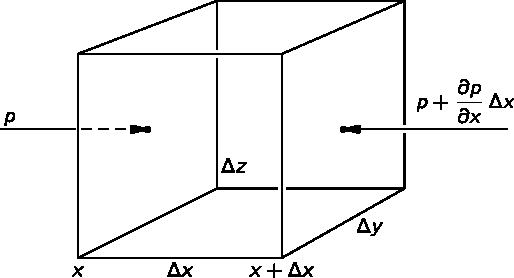
\includegraphics[width=0.7\linewidth]{fyz_fig546.pdf}
      \caption{Výsledná hustota tlakové síly na krychli je \(\symbf{\nabla} p\)
               (\cite[s.~742]{Feynman02})}
      \label{fyz_fig546}
    \end{figure}
    
    Vezměme si případ, kdy takovou dodatečnou sílu lze popsat pomocí potenciální energie, jako je 
    to v případě gravitace; \(\varphi\) bude označovat potenciální energii na jednotku hmotnosti. 
    (V případě gravitace je např. \(\varphi\) právě \(gz\).) Síla na jednotku hmotnosti se pomocí 
    potenciálu vyjadřuje jako \(-\symbf{\nabla}\varphi\) a je-li \(\varrho\) hustota kapaliny, bude 
    síla na jednotku objemu \(-\varrho\bmod{\nabla}\varphi\). V rovnováze musí být součet této 
    hustoty síly a hustoty tlakové síly nulový:
    \begin{equation}\label{fyz:eq546}
      - \symbf{\nabla} p - \varrho\symbf{\nabla}\varphi = 0.
    \end{equation}
    
    Rovnice (\ref{fyz:eq546}) je \emph{rovnicí hydrostatiky}. Obecně \emph{nemá} řešení. Pokud se 
    hustota v prostoru mění libovolným způsobem, síly se nijak nemohou vyrovnat a kapalina se 
    nemůže nacházet ve stabilní rovnováze. Začnou téci konvekční proudy. Můžeme to vidět přímo z 
    rovnice, neboť tlakový člen je úplným gradientem, zatímco druhý člen ne, neboť obsahuje i 
    proměnnou hustotu \(\varrho\). Pouze je-li \(\varrho\) konstantní, je i potenciální člen úplným 
    gradientem. Pak je řešením rovnice
    \begin{equation*}
      p + \varrho\varphi = \text{konst}. 
    \end{equation*}
    
    Jiná možnost vzniku hydrostatické rovnováhy je případ, kdy \(\varrho\) je jen funkcí \(p\). 
    Opusťme však hydrostatiku, neboť není ani zdaleka tak zajímavá jako situace, kdy jsou kapaliny 
    v pohybu.
    
  \section{Pohybové rovnice}\label{fyz:IIchapXLsecII}
    Nejdříve prodiskutujeme pohyb tekutin z čistě abstraktního, teoretického hlediska a pak si 
    všimneme několika speciálních případů. Abychom popsali pohyb kapaliny, musíme zadat její 
    vlastnosti v každém bodě. Například v různých místech se voda (nazývejme naší kapalinu vodou) 
    pohybuje různými rychlostmi. Abychom specifikovali charakter proudění, musíme v každém bodě a v 
    každém čase zadat tři složky \emph{rychlosti}. Dokážeme-li zformulovat rovnice, které určují 
    rychlost, budeme vědět, jak se kapalina v každém okamžiku pohybuje. Rychlost však není jedinou 
    vlastností kapaliny, která se mění od místa k místu. Právě před chvílí jsme hovořili o změnách 
    \emph{tlaku}. A existují i další proměnné veličiny. Od bodu k bodu se může měnit i 
    \emph{hustota}. Navíc kapalina může být i vodičem a vést elektrický \emph{proud}, jehož hustota 
    \(\vec{j}\) mění od bodu k bodu svou velikosti směr. Měnit se může i teplota, magnetické pole 
    atd. Počet polí, které potřebujeme k popisu úplné situace, závisí na tom, jak komplikovaný je 
    studovaný problém. Dochází k zajímavým jevům, kdy dominantní úlohu při určování chování 
    kapaliny hrají proudy a magnetizmus; to je tématem \textbf{magnetohydrodynamiky}. Takových 
    složitějších situací si však nebudeme všímat, neboť už na nižší úrovni existuje řada zajímavých 
    jevů a i tato elementární úroveň bude dost komplikovaná. 
    
    Zvažme situaci, v níž nevystupuje magnetické pole ani vodivost, a nebudeme se starat ani o 
    teplotu, neboť budeme předpokládat, že teplota v libovolném bodě je jednoznačně určena hustotou 
    a tlakem. Dokonce si práci zjednodušíme předpokladem, že hustota je konstantní - budeme si 
    představovat, že kapalina je v podstatě nestlačitelná. Jinými slovy, předpokládáme, že změny 
    tlaku jsou tak malé, že jimi způsobené změny jsou zanedbatelné. Kdyby to tak nebylo, museli 
    bychom vzít v úvahu další jevy, např. šíření zvuku nebo rázových vln. Šíření zvuku a rázových 
    vln jsme už do jisté míry probrali, proto nyní náš rozbor hydrodynamiky od těchto jevů 
    izolujeme a budeme předpokládat, že hustota \(\varrho\) je konstantní. Je snadné určit, kdy je 
    přiblížení konstantního \(\varrho\) dobré. Můžeme říci, že pokud jsou rychlosti proudění mnohem 
    menší než rychlost zvukové vlny v kapalině, nemusíme se o změny hustoty zajímat. To, jak voda 
    uniká našim pokusům pochopit její chování, nesouvisí s přiblížením konstantní hustoty. 
    Komplikace, které její únik umožňují, probereme v následující kapitole. 
    
    Obecnou teorii tekutin musíme začít od \textbf{stavové rovnice}, která udává souvislost tlaku a 
    hustoty. V našem přiblížení je tato stavová rovnice jednoduchá:
    \begin{equation*}
      \varrho = \text{konst}.
    \end{equation*}
    To je první vztah pro naše proměnné. Další vztah vyjadřuje zachování látky: Odtéká-li látka z 
    nějakého místa, musí se množství látky, které v daném místě zůstává zmenšit. S podobným vztahem 
    jsme se setkali u elektřiny. Odtud také víme, že divergence takové veličiny udává rychlost 
    poklesu hustoty za jednotku času. Podobně rovnice
    \begin{equation}\label{fyz:eq547}
      \symbf{\nabla}\cdot(\varrho v) = -\pder{\varrho}{t}
    \end{equation}
    vyjadřuje zachování hmotnosti tekutiny; je to hydrodynamická \textbf{rovnice kontinuity}. V 
    našem přiblížení nestlačitelné tekutiny je \(\varrho\) konstantní a rovnice kontinuity má 
    jednoduchý tvar
    \begin{equation}\label{fyz:eq548}
      \symbf{\nabla}\cdot\bm{v} = 0.
    \end{equation}
    Rychlost tekutiny \(\bm{v}\) (podobně jako magnetická indukce \(\bm{B}\)) má nulovou 
    divergenci. (Rovnice hydrodynamiky jsou často analogické s rovnicemi elektrodynamiky, proto 
    jsme studovali nejdříve elektrodynamiku. Někteří lidé mají jiný názor; myslí si, že je nutné 
    nejdříve studovat hydrodynamiku, takže je pak snazší porozumět elektrodynamice. Elektrodynamika 
    je ale ve skutečnosti mnohem snazší než hydrodynamika)
    
    Další rovnici získáme z Newtonova zákona, který nám říká, jak se rychlost mění v důsledku 
    působících sil. Hmotnost objemového elementu kapaliny krát jeho zrychlení musí být rovno síle, 
    která na element působí. Vybereme-li element s jednotkovým objemem a označíme-li sílu na 
    jednotku objemu jako \(f\) platí
    \begin{equation*}
      \varrho\times\text{zrychlení} = \bm{f}.
    \end{equation*}
    Hustotu síly zapíšeme jako součet tří členů. Už jsme zmínili tlakovou sílu na jednotku objemu, 
    \(-\symbf{\nabla}p\). Dále existují vnější síly, které působí na dálku, např. gravitace nebo 
    elektřina. Jsou-li to konzervativní síly, jejichž potenciál na jednotku hmotnosti je 
    \(\varphi\), odpovídá jim hustota síly \(\varrho\symbf{\nabla}\varphi\). (Kdyby vnější síly 
    nebyly konzervativní, museli bychom za hustotu vnější síly psát \(\bm{f_{\text{vněj}}}\).) 
    Existuje ještě jiná, vnitřní síla na jednotku objemu, která souvisí se skutečností, že v 
    \emph{proudící} tekutině mohou existovat smyková napětí. Nazývá se viskózní síla; označíme ji 
    \(\bm{f_{\text{visk}}}\). Naše pohybová rovnice Je
    \begin{equation}\label{fyz:eq549}
      \varrho\times\text{zrychlení} = 
        \symbf{\nabla}p - \varrho\symbf{\nabla}\varphi + \bm{f_{visk}}.
    \end{equation}
    
    V této kapitole budeme předpokládat, že tekutina je řídká v tom smyslu, že viskozita není 
    důležitá, a vynecháme \(\bm{f_{\text{visk}}}\). Vynecháme-li viskozitu, provádíme 
    přiblížení, které popisuje nějakou ideální látku, a ne skutečnou vodu. John von Neumann si 
    svého času byl dobře vědom obrovského rozdílu mezi chováním tekutiny, vynecháme-li resp. 
    zahrneme-li viskózní členy, a byl si také vědom skutečnosti, že po dobu téměř celého vývoje 
    hydrodynamiky přibližně do roku \num{1900} se většina zájmu koncentrovala na řešení krásných 
    \emph{matematických} problémů, které neměly téměř nic společného se skutečnými tekutinami. 
    Proto teoretiky, kteří se zabývali takovými analýzami, nazval lidmi, kteří studují „suchou 
    vodu“. Takové analýzy vynechávají \emph{podstatnou} vlastnost tekutin. Jelikož i my v této 
    kapitole v našich výpočtech tuto vlastnost zanedbáváme, nazvali jsme ji „Proudění suché vody“. 
    Diskuzi \emph{skutečné} vody odložíme do následující kapitoly.
    
    \begin{figure}[ht!] %\ref{fyz_fig547}
      \centering
      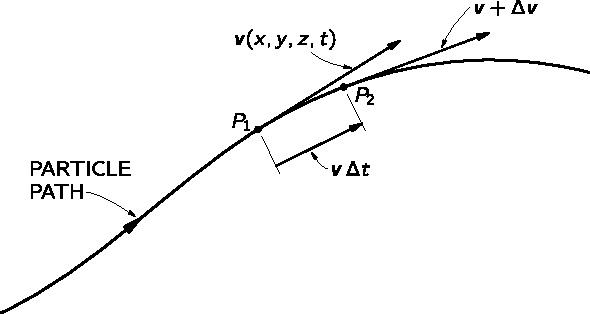
\includegraphics[width=0.7\linewidth]{fyz_fig547.pdf}
      \caption{Zrychlení částice kapaliny
               (\cite[s.~744]{Feynman02})}
      \label{fyz_fig547}
    \end{figure}
    
    Vynecháme-li \(f_{\text{visk}}\), máme v rovnici (\ref{fyz:eq549}) vše potřebné kromě výrazu 
    pro zrychlení. Mohli bychom si myslet, že vzorec pro zrychlení částice kapaliny bude velmi 
    jednoduchý, neboť se zdá zřejmé, že je-li \(v\) rychlost částice v některém místě tekutiny, je 
    zrychlení pouze \(\pder{\bm{v}}{t}\). \emph{Není}, a důvod pro to je dost rafinovaný. Derivace 
    \(\pder{\bm{v}}{t}\) je rychlost, jíž se rychlost \(v(x, y, z, t)\) mění v \emph{pevném bodě} 
    prostoru. My však potřebujeme vědět, jak rychle se mění rychlost určité části tekutiny. 
    Představte si, že obarvíme kapku vody, abychom ji mohli pozorovat. Za malý čas \(\Delta t\) se 
    tato kapka přesune na jiné místo. Pohybuje-li se kapka podél nějaké trajektorie jako na obr. 
    \ref{fyz_fig547}, za čas \(\Delta t\) se například přesune z bodu \(P_1\) do bodu \(P_2\). Ve 
    směru osy \(x\) se posune o \(v_x\Delta t\), ve směru osy \(у\) о \(v_y\Delta t\) a ve směru 
    osy \(z\) o \(v_z\Delta t\). Vidíme, že je-li \(v(x, y, z, t)\) rychlost částice v tekutině v 
    bodě \((x, y, z)\) v čase \(t\), má tatáž částice v čase \(t + \Delta t\) rychlost \(v(x+ 
    \Delta x, y + \Delta y, z + \Delta z, t + \Delta t)\), přičemž
    \begin{equation*}
      \Delta x = v_x\Delta t, \qquad  \Delta y = v_y\Delta t, \qquad  \Delta z = v_z\Delta t.
    \end{equation*}
    
    Podle definice parciálních derivací (vzpomeňte si na rovnici (\ref{fyz:eq245})) s přesností 
    prvního řádu
    \begin{align*}
      \bm{v}(x+ \Delta x, y 
        &+ \Delta y, z + \Delta z, t + \Delta t) 
         = \bm{v}(x, y, z, t)                                                                \\
        &+ \pder{\bm{v}}{x}v_x\Delta t + \pder{\bm{v}}{y}v_y\Delta t + \pder{\bm{v}}{z}v_z\Delta t
         + \pder{\bm{v}}{t}\Delta t.
    \end{align*}
    Zrychlení \(\Delta{\bm{v}}/\Delta{t}\) je pak rovno
    \begin{equation*}
      \pder{\bm{v}}{x}v_x + \pder{\bm{v}}{y}v_y + \pder{\bm{v}}{z}v_z + \pder{\bm{v}}{t}.
    \end{equation*}
    Zacházíme-li s \(\bm{v}\) jako s vektorem, můžeme poslední vztah zapsat symbolicky
    \begin{equation}\label{fyz:eq550}
      (\bm{v}\cdot\symbf{\nabla})\bm{v} + \pder{\bm{v}}{t}.
    \end{equation}
    Všimněte si, že zrychlení může být nenulové i tehdy, když \(\pder{\bm{v}}{t} = 0\), tj. když se 
    rychlost \emph{v daném bodě} nemění. Uveďme příklad: Voda, která teče po kružnici konstantní 
    rychlostí, se zrychluje, ačkoliv se rychlost v daném bodě nemění. Důvodem samozřejmě je, že 
    rychlost vybraného množství vody, které se původně nacházelo v jednom bodě na kružnici, má za 
    okamžik jiný směr; působí na ni dostředivé zrychlení. 
    
    Zbytek naší teorie je čistá matematika - je nutné najít řešení pohybových rovnic, které 
    dostaneme, dosadíme-li zrychlení (\ref{fyz:eq551}) do rovnice (\ref{fyz:eq550}). Platí
    \begin{equation}\label{fyz:eq551}
      (\bm{v}\cdot\symbf{\nabla})\bm{v}+\pder{\bm{v}}{t} 
        = -\dfrac{\symbf{\nabla}p}{\varrho} -\symbf{\nabla}\varphi.
    \end{equation}
    přičemž jsme viskozitu vynechali. Tuto rovnici můžeme přepsat na jiný tvar, využijeme-li 
    následující identity z vektorové analýzy:
    \begin{equation*}
      (\bm{v}\cdot\symbf{\nabla})\bm{v} 
        = (\symbf{\nabla}\times\bm{v})\times\bm{v} + \frac{1}{2}\symbf{\nabla}(\bm{v}\cdot\bm{v}).
    \end{equation*}
    Definujeme-li nyní rotaci \(\bm{v}\) jako nové vektorové pole \(\symbf{\Omega}\)  
    \begin{equation}\label{fyz:eq552}
      \symbf{\Omega} = \symbf{\nabla}\times\bm{v},
    \end{equation}
    lze vektorovou identitu přepsat na
    \begin{equation*}
      (\bm{v}\cdot\symbf{\nabla})\bm{v} 
        = \symbf{\Omega}\times\bm{v} + \frac{1}{2}\symbf{\nabla}v^2,
    \end{equation*}
    a naše pohybová rovnice (\ref{fyz:eq551}) se změní na
    \begin{equation}\label{fyz:eq553}
      \pder{\bm{v}}{t} + \symbf{\Omega}\times\bm{v} + \frac{1}{2}\symbf{\nabla}v^2
        = -\dfrac{\symbf{\nabla}p}{\varrho} -\symbf{\nabla}\varphi.
    \end{equation}
    
    Ekvivalence rovnic (\ref{fyz:eq551}) a (\ref{fyz:eq553}) si můžeme ověřit tak, že je přepíšeme 
    do složek a porovnáme, přičemž využijeme vztah (\ref{fyz:eq552}).
    
    Vektorové pole \(\symbf{\Omega}\) se nazývá \textbf{vírnatost}. Je-li \(\symbf{\Omega}\) všude 
    rovno nule, proudění nazýváme nevířivým. V článku \ref{fyz:IIchapIIIsecIV} jsme zavedli 
    cirkulaci vektorového pole. Cirkulace podél uzavřené smyčky v kapalině je křivkový integrál 
    rychlosti kapaliny (v daném časovém okamžiku) podél smyčky:
    \begin{equation*}
      \text{cirkulace} = \oint\bm{v}\cdot\bm{ds}
    \end{equation*}
    Cirkulace na \emph{jednotku plochy} infinitesimální smyčky je pak podle Stokesovy věty rovna 
    \(\symbf{\nabla}\times\bm{v}\). Vektor \(\symbf{\Omega}\) tedy udává cirkulaci kolem jednotkové 
    plochy (kolmé na směr \(\symbf{\Omega}\)). Kromě toho je zřejmé, že vložíme-li na libovolné 
    místo v kapalině kousek nečistoty (neinfinitesimálně malý), bude se otáčet úhlovou rychlostí 
    \(\symbf{\Omega}/2\). Také můžeme dokázat, že v případě vědra s vodou na otočném stolku je 
    \(\symbf{\Omega}\) rovno dvojnásobku lokální úhlové rychlosti vody.
    
    Zajímáme-li se jen o pole rychlostí, můžeme z našich rovnic vyloučit tlak. Vypočítáme-li rotaci 
    obou stran rovnice (\ref{fyz:eq553}), vzpomeneme si, že \(\varrho\) je konstantní a rotace 
    libovolného gradientu je nulová, a použijeme vztah (\ref{fyz:eq548}), dostaneme
    \begin{equation}\label{fyz:eq554}
      \pder{\symbf{\Omega}}{t} + \symbf{\nabla}\times(\symbf{\Omega}\times\bm{v}) = 0.
    \end{equation}
    Tato rovnice spolu s rovnicemi
    \begin{equation}\label{fyz:eq555}
      \symbf{\Omega} = \symbf{\nabla}\times\bm{v}
    \end{equation}
    a
    \begin{equation}\label{fyz:eq556}
      \symbf{\nabla}\cdot\bm{v} = 0.
    \end{equation}
    úplně popisuje pole rychlostí \(\bm{v}\). Matematicky řečeno, známe-li v nějakém čase 
    \(\symbf{\Omega}\) známe i rotaci vektoru rychlosti. Dále víme, že jeho divergence je nulová, 
    takže v dané fyzikální situaci máme vše potřebné k určení \(\bm{v}\) v celém prostoru. (Se 
    stejnou situací jsme se setkali v magnetizmu, kde \(\symbf{\nabla}\cdot\bm{B}=0\) a 
    \(\symbf{\nabla}\times\bm{B}=\bm{j}/\varepsilon_0c^2\).) Zadání \(\symbf{\Omega}\) určuje 
    \(\bm{v}\) podobně jako zadání \(\bm{j}\) určuje \(\bm{B}\). Známe-li \(\bm{v}\), rovnice 
    (\ref{fyz:eq554}) nám poví, jaká je rychlost změny \(\symbf{\Omega}\) a zní opět najdeme nové 
    \(\bm{v}\) atd. Vidíme, že tyto rovnice obsahují vše potřebné pro výpočet rychlosti proudění. 
    Uvědomme si však, že tato procedura poskytuje jen pole rychlostí; celou informaci o tlaku jsme 
    ztratili. 
    
    Uveďme jeden speciální důsledek našich rovnic. Je-li \(\symbf{\Omega}=0\) všude v nějakém čase 
    \(t\), je \(\pder{\symbf{\Omega}}{t}\) také nulové, takže \(\symbf{\Omega}\) je nulové i v čase 
    \(t + \Delta t\). Řešením naší rovnice je tedy proudění, které je neustále, v každém čase, 
    nevířivé. Začalo-li pole s nulovou rotací, bude mít nulovou rotaci vždy. Pak je třeba vyřešit 
    rovnice
    \begin{equation*}
      \symbf{\nabla}\cdot\bm{v} = 0, \qquad \symbf{\nabla}\times\bm{v} = 0
    \end{equation*}
    Připomínají rovnice pro elektrostatické a magnetické pole v prázdném prostoru. Později se k nim 
    vrátíme a podíváme se na několik konkrétních příkladů.
    
  \section{Ustálené proudění - Bernoulliova věta}\label{fyz:IIchapXLsecIII}
    Nyní se vrátíme k pohybovým rovnicím (\ref{fyz:eq553}), ale omezíme se na případy ustáleného 
    proudění. Ustáleným prouděním rozumíme to, že se na žádném místě tekutiny rychlost nikdy 
    nemění. Tekutina v libovolném bodě je vždy nahrazena novou tekutinou, která proudí přesně 
    stejným způsobem. Rychlosti vypadají stále stejně, \(\bm{v}\) je statické vektorové pole. 
    Podobně jako jsme kreslili siločáry v magnetostatice, můžeme nyní kreslit čáry, k nimž je 
    rychlost neustále tečnou, jak to znázorňuje obr. \ref{fyz_fig547}. Tyto čáry se nazývají 
    \textbf{proudnice}. V případě ustáleného proudění jsou to skutečné trajektorie částic tekutiny. 
    (Při neustáleném proudění se proudnicový obraz mění v čase a proudnice v žádném okamžiku 
    nepředstavují trajektorii částice tekutiny.)
    
    \begin{figure}[ht!] %\ref{fyz_fig547}
      \centering
      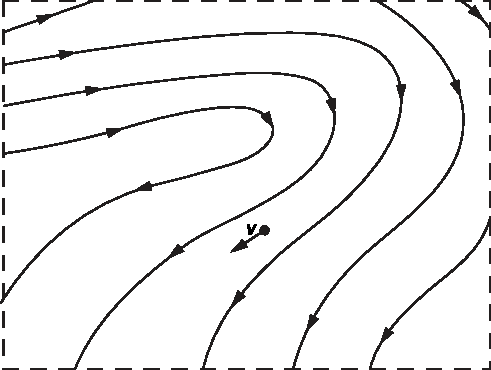
\includegraphics[width=0.7\linewidth]{fyz_fig548.pdf}
      \caption{Proudnice při ustáleném proudění kapaliny
               (\cite[s.~747]{Feynman02})}
      \label{fyz_fig548}
    \end{figure}
    
    Ustálené proudění neznamená, že se neděje vůbec nic: atomy v tekutině se pohybují a mění
    své rychlosti. Platí jen \(\pder{\bm{v}}{t} = 0\). Vypočítáme-li pak skalární součin \(\bm{v}\) 
    v rovnici pohybu, člen \(\bm{v}\cdot(\symbf{\Omega}\times\bm{v})\)  vypadne a zůstane nám
    \begin{equation}\label{fyz:eq557}
      \bm{v}\cdot\symbf{\nabla}\left\lbrace\dfrac{p}{\varrho}
      + \varphi + \dfrac{1}{2}v^2\right\rbrace = 0.
    \end{equation}
    Tato rovnice nám říká, že při malých posunutích ve směru rychlosti tekutiny se veličina ve 
    složené závorce nemění. V případě ustáleného proudění se všechna posunutí dějí podél proudnic, 
    takže rovnice (\ref{fyz:eq557}) zároveň říká, že \emph{pro všechny body podél proudnice} platí
    \begin{equation}\label{fyz:eq558}
      \dfrac{p}{\varrho}+\varphi+\dfrac{1}{2}v^2 = \text{konst} \qquad \text{(na proudnici)}.
    \end{equation}
    Je to takzvaná \textbf{Bernoulliova věta}. Konstanta na pravé straně může být obecně pro různé 
    proudnice různá; víme jen, že levá strana rovnice (\ref{fyz:eq558}) je podél dané proudnice 
    konstantní. Můžeme si však všimnout, že v případě ustáleného nevířivého proudění, při němž 
    \(\symbf{\Omega} =0\), nám pohybová rovnice (\ref{fyz:eq553}) poskytuje vztah
    \begin{equation}\label{fyz:eq559}
      \symbf{\nabla}\left\lbrace\dfrac{p}{\varrho}+\varphi+\dfrac{1}{2}v^2\right\rbrace = 0,
    \end{equation}
    takže
    \begin{equation}\label{fyz:eq560}
      \dfrac{p}{\varrho}+\varphi+\dfrac{1}{2}v^2 = \text{konst} \qquad \text{(všude)}.
    \end{equation}
    Vztah je stejný jako (\ref{fyz:eq558}) ale nyní musí mít konstanta \emph{stejnou hodnotu v celé 
    tekutině}.

    \begin{figure}[ht!]
      \centering
      \begin{tabular}{c}
        \subfloat[ ]{\label{fyz_fig549a}
          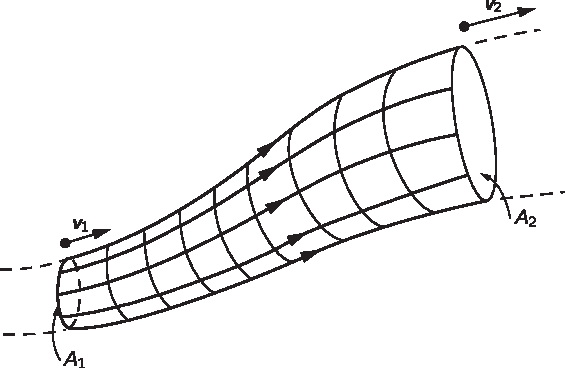
\includegraphics[width=0.7\linewidth]{fyz_fig549a.pdf}}               \\
        \subfloat[ ]{\label{fyz_fig549b}
          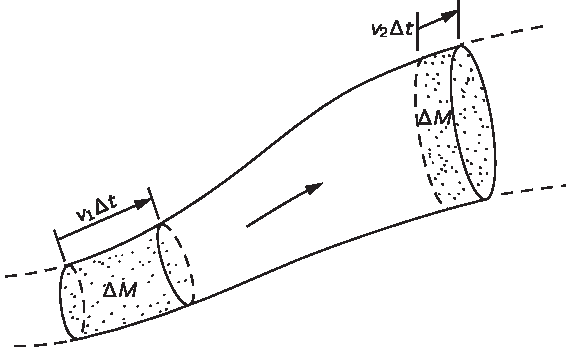
\includegraphics[width=0.7\linewidth]{fyz_fig549b.pdf}}              
      \end{tabular}
      \caption{Pohyb tekutiny v proudové trubici
               (\cite[s.~748]{Feynman02})}
    \end{figure}
    
    Bernoulliova věta není ve skutečnosti nic jiného než tvrzení o zachování energie. Taková věta o 
    zachování energie nám poskytuje mnoho informací o proudění, aniž bychom skutečně našli detailní 
    řešení rovnic. Bernoulliova věta je natolik důležitá a natolik jednoduchá, že si ukážeme ještě 
    jeden způsob jejího odvození, který se liší od formálních výpočtů, jaké jsme provedli dosud. 
    Představme si svazek blízkých proudnic, které vytvářejí proudovou trubici jako na obr. 
    \ref{fyz_fig549a}. Jelikož jsou stěny trubice vytvořeny z proudnic, nevytéká jimi žádná 
    tekutina. Nazvěme průřez na jednom konci proudové trubice \(S_1\), rychlost tekutiny v tomto 
    průřezu \(v_1\), hustotu tekutiny \(\varrho_1\), a potenciální energii  \(\varphi_1\). 
    Odpovídající veličiny na druhém konci trubice jsou \(S_2\), \(v_2\), \(\varrho_2\), a 
    \(\varphi_2\). Za krátký časový úsek \(\Delta t\) se kapalina v \(S_1\) posunula o vzdálenost 
    \(v_1\Delta t\) a tekutina v \(S_2\), o vzdálenost \(v_2\Delta t\) (obr. \ref{fyz_fig549b}). 
    Zachování hmotnosti vyžaduje, aby hmotnost, která vejde do trubice koncem \(S_1\), byla rovna 
    hmotnosti, která z ní vyjde koncem \(S_2\). Tyto hmotnosti musí být na obou koncích stejné:
    \begin{equation*}
      \Delta M = \varrho_1S_1v_1\Delta t = \varrho_2S_2v_2\Delta t.
    \end{equation*}
    Máme tedy rovnost
    \begin{equation}\label{fyz:eq561}
      \varrho_1S_1v_1\Delta t = \varrho_2S_2v_2\Delta t.
    \end{equation}
    Tato rovnice nám říká, že při konstantní hustotě se rychlost mění nepřímo úměrně průřezu 
    proudové trubice
    
    Nyní vypočítáme práci, kterou vykonal tlak v tekutině. Práce vykonaná na tekutině, která vtéká 
    do \(S_1\) je \(p_1S_1v_1\Delta t\), zatímco práce odevzdaná v \(S_2\) je \(p_2S_2v_2\Delta 
    t\). Výsledná práce vykonaná na tekutině mezi \(S_1\) a \(S_2\) je proto
    \begin{equation*}
      p_1S_1v_1\Delta t - p_2S_2v_2\Delta t
    \end{equation*}
    a musí být rovna zvýšení energie hmotnosti \(\Delta M\) tekutiny při přechodu z \(S_1\) do 
    \(S_2\), Jinými slovy:
    \begin{equation}\label{fyz:eq562}
      p_1S_1v_1\Delta t - p_2S_2v_2\Delta t = \Delta M(E_2 - E_1),
    \end{equation}
    přičemž \(E_1\) je energie na jednotku hmotnosti tekutiny v \(S_1\) a \(E_2\), energie na 
    jednotku hmotnosti na \(S_2\). Energii na jednotku hmotnosti tekutiny můžeme zapsat jako
    \begin{equation*}
      E = \dfrac{1}{2}v^2 + \varphi + W,
    \end{equation*}
    kde \(v^2/2\) je kinetická energie na jednotku hmotnosti, \(\varphi\) je potenciální energie na 
    jednotku hmotnosti a \(W\) je dodatečný člen, který reprezentuje vnitřní energii jednotky 
    hmotnosti tekutin. Vnitřní energie může odpovídat například tepelné energii stlačitelné 
    tekutiny nebo chemické energii. Všechny tyto veličiny se od místa k místu mění. Využijeme-li 
    vztah pro energii v (\ref{fyz:eq562}), vyjde
    \begin{equation*}
      \dfrac{p_1S_1v_1\Delta t}{\Delta M} - \dfrac{p_2S_1v_2\Delta t}{\Delta M} = 
        \dfrac{1}{2}v_2^2 + \varphi_2 + W_2 - \dfrac{1}{2}v_1^2 - \varphi_1 - W_1.
    \end{equation*}
    Už jsme však viděli, že \(\Delta M= \varrho Sv\Delta t\), takže dostaneme
    \begin{equation}\label{fyz:eq563}
      \dfrac{p_1}{\varrho_1} + \dfrac{1}{2}v_1^2 + \varphi_1 + W_1 
        = \dfrac{p_2}{\varrho_2} + \dfrac{1}{2}v_2^2 + \varphi_2 + W_2,
    \end{equation}
    což je Bernoulliův výsledek s dodatečným členem za vnitřní energii. Je-li tekutina 
    nestlačitelná, vnitřní energie je na obou stranách rovnice stejná a opět vychází, že podél 
    každé proudnice platí vztah (\ref{fyz:eq560}).
    
    \begin{figure}[ht!] %\ref{fyz_fig550}
      \centering
      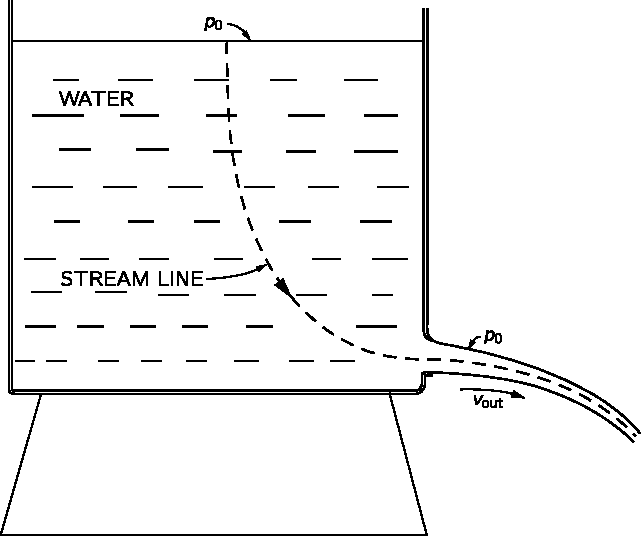
\includegraphics[width=0.6\linewidth]{fyz_fig550.pdf}
      \caption{Proudění z nádrže
               (\cite[s.~749]{Feynman02})}
      \label{fyz_fig550}
    \end{figure}

    Nyní si všimneme několika jednoduchých příkladů, v nichž nám Bernoulliovo řešení umožňuje najít 
    proudění. Nechť voda vytéká z otvoru u dna nádrže, jak je nakresleno na obr. \ref{fyz_fig550}. 
    Uvažme situaci, v níž je rychlost proudění \(v_{\text{výt}}\) u otvoru mnohem větší než 
    rychlost proudění u hladiny nádrže; jinými slovy předpokládáme, že průměr nádrže je tak velký, 
    že můžeme zanedbat pokles hladiny tekutiny. (Kdybychom chtěli, mohli bychom uskutečnit i 
    přesnější výpočet). U hladiny je tlak \(p_0\), tj. \emph{atmosférický tlak}; stejný je i tlak, 
    který působí na vytékající proud tekutiny. Napíšeme Bernoulliovu rovnici pro některou z 
    proudnic, např. takovou jaká je zobrazena na obrázku. U hladiny nádrže vezmeme \(v = 0\) a také 
    gravitační potenciál \(\varphi = 0\). U otvoru je rychlost \(v_{\text{výt}}\) a \(\varphi= 
    -gh\), a tedy
    \begin{align}
      p_0 &= p_0 + \dfrac{1}{2}\varrho v_{\text{výt}}^2 - \varrho gh \nonumber \\
      \shortintertext{resp.}
      v_{\text{výt}} &= \sqrt{2gh}.                                   \label{fyz:eq564}
    \end{align}
    To je stejná rychlost jako rychlost tělesa padajícího z výšky \(h\). Příliš nás to 
    nepřekvapuje, neboť voda u otvoru získala kinetickou energii na úkor potenciální energie vody u 
    hladiny. Nemysleme si však, že rychlost ubývání tekutiny v nádrži vypočítáme tak, že tuto 
    rychlost vynásobíme velikostí plochy otvoru. V místě, kde proud tekutiny opouští otvor, nejsou 
    rychlosti rovnoběžné, ale mají složky, které směřují dovnitř proudu - proud je sbíhavý. Když 
    proud trochu postoupí, zužování se zastaví a rychlosti jsou opět rovnoběžné. Celkový výtok je 
    tedy roven rychlost krát průřez v tomto místě. Opravdu, má-li výtokový otvor tvar kruhu s 
    ostrým okrajem, zúží se proud na \num{62} procent plochy průřezu otvoru. Redukovaná efektivní 
    plocha výtoku se mění pro různé tvary výtokových trubic a její experimentální hodnotu lze najít 
    v tabulkách \emph{výtokových koeficientů}.
    
    Je-li výtoková trubice vsunuta dovnitř tekutiny jako na obr. \ref{fyz_fig551}, lze velmi krásně 
    dokázat, že výtokový koeficient je přesně \SI{50}{\percent}. Zde jen naznačíme, jak důkaz 
    probíhá. Pro určení rychlosti (viz vztah (\ref{fyz:eq564})) jsme využili zachování energie, je 
    však ještě nutné zvážiti zachování hybnosti.
    
    \begin{figure}[ht!] %\ref{fyz_fig551}
      \centering
      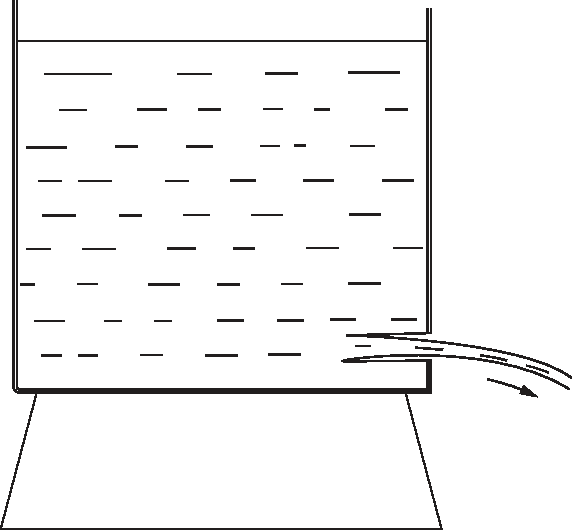
\includegraphics[width=0.6\linewidth]{fyz_fig551.pdf}
      \caption{Je-li výtoková trubice vsunuta dovnitř nádoby, je proud zúžen na polovinu plochy 
               průřezu
               (\cite[s.~750]{Feynman02})}
      \label{fyz_fig551}
    \end{figure}
    
    Jelikož s vytékajícím proudem odtéká i hybnost, na průřezu výtokové trubice musí působit nějaká 
    síla. Odkud se tato síla bere? Síla musí pocházet z tlaku na stěny. Pokud je výtokový otvor 
    malý a daleko od stěn, bude rychlost kapaliny blízko stěn nádrže velmi malá. Tlak na každou 
    stěnu je proto stejný jako statický tlak v nehybné tekutině, viz vztah (\ref{fyz:eq560}). Pak 
    musí být statický tlak v libovolném bodě na jedné straně nádrže kompenzován stejným tlakem v 
    bodě na protilehlé straně s \emph{výjimkou} bodů na stěně, které leží proti výtokové trubici. 
    Vypočítáme-li hybnost, která je „vypuzena“ tímto tlakem spolu s proudem tekutiny, zjistíme, že 
    výtokový koeficient je \num{1/2}. Tento způsob výpočtu nemůžeme použít v případě výtokového 
    otvoru na obr. \ref{fyz_fig550}, neboť zvýšení rychlosti u stěny v blízkosti výtokového otvoru 
    způsobuje pokles tlaku, který neumíme vypočítat.

    \begin{figure}[ht!] %\ref{fyz_fig552}
      \centering
      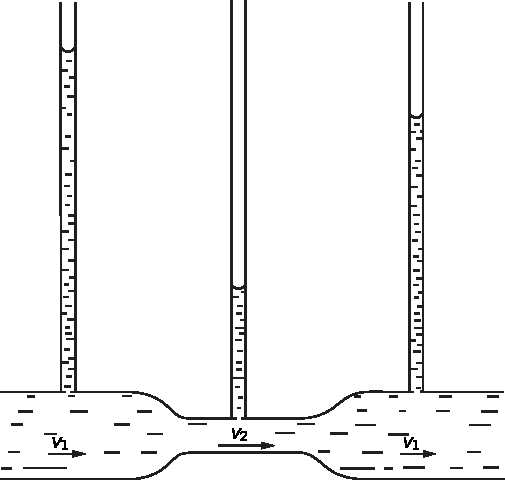
\includegraphics[width=0.6\linewidth]{fyz_fig552.pdf}
      \caption{Tlak je nejnižší, když je rychlost nejvyšší
               (\cite[s.~751]{Feynman02})}
      \label{fyz_fig552}
    \end{figure}
    
    Nyní se podívejme na jiný příklad, na vodovodní trubku s proměnným průřezem jako na obr. 
    \ref{fyz_fig553}, do níž vtéká voda jedním koncem a druhým vytéká. Zachování energie, tj. 
    Bernoulliova rovnice, nám říká, že tlak je nižší ve zúžené oblasti, kde je větší rychlost. 
    Tento efekt můžeme snadno demonstrovat, změříme-li tlaky v různých průřezech pomocí malých 
    svislých sloupců vody, které jsou k proudové trubici připojeny tak malými otvory, že nenarušují 
    charakter proudění. V takovém případě je tlak úměrný výšce vody v těchto svislých sloupcích. 
    Zjistíme, že tlak v místě zúžení je nižší než na obou rozšířených stranách. Vrátí-li se 
    velikost průřezu za místem zúžení na původní hodnotu před zúžením, tlak opět vzroste. 
    Bernoulliův vztah předpovídá, že tlak za zúženým místem bude stejný jako předtím, ve 
    skutečnosti je však viditelně menší. Důvod nesprávnosti naší předpovědi je ten, že jsme 
    zanedbali třecí, viskózní síly, které způsobují pokles tlaku podél trubky. Přes tento pokles 
    tlaku je tlak ve zúženém místě zaručeně nižší (vzhledem k větší rychlosti) než v obou širších 
    místech souhlasně s Bernoulliovou předpovědí. Rychlost \(v_2\) zaručeně musí převýšit \(v_1\) 
    proteklo-li stejné množství zúženým místem. Voda je tedy při průchodu ze širšího místa do 
    užšího zrychlována. Síla, která toto zrychlení způsobuje, pochází z poklesu tlaku.
    
    \begin{figure}[ht!] %\ref{fyz_fig553}
      \centering
      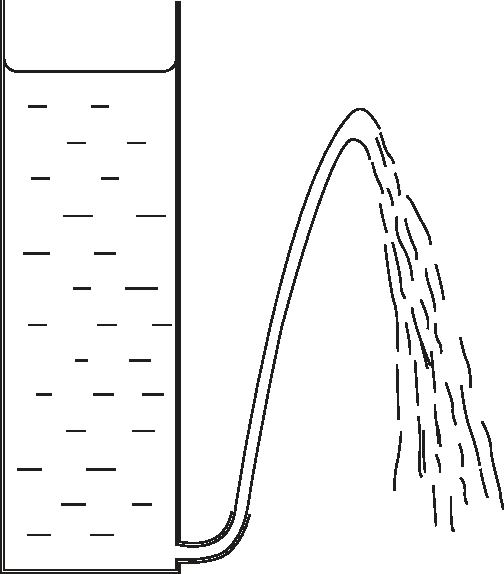
\includegraphics[width=0.6\linewidth]{fyz_fig553.pdf}
      \caption{Důkaz, že \(v\) není rovno \(\sqrt{2gh}\)
               (\cite[s.~751]{Feynman02})}
      \label{fyz_fig553}
    \end{figure}
    
    Naše výsledky můžeme ověřit ještě v jednom jednoduchém pokusu. Představme si, že máme nádrž s 
    výtokovou trubicí, která vrhá proud vody směrem nahoru, jak je ukázáno na obr. 
    \ref{fyz_fig553}. Kdyby byla výtoková rychlost přesně \(\sqrt{2gh}\), musela by vytékající vody 
    vystoupit do stejné výšky, v jaké se nachází hladina vody v nádrži. V experimentu až tam 
    nevystoupí. Naše předpověď je přibližně správná, ale opět viskózní tření, které jsme nezahrnuli 
    do našeho vzorce pro zachování energie, způsobilo energetické ztráty.
    
    Drželi jste někdy u sebe dva listy papíru a zkusili jste je oddělit fouknutím? Zkuste to! Vrátí 
    se k \emph{sobě}. Důvodem je, samozřejmě, že vzduch má \emph{vyšší} rychlost, když prochází 
    zúženým prostorem mezi listy, než když je mimo. Tlak mezi listy je \emph{nižší} než 
    atmosférický tlak, a tak k sobě listy přilnou, místo aby se vzdálili.
    
  \section{Vířivé proudění}\label{fyz:IIchapXLsecIV}
    Na začátku předcházejícího článku jsme zjistili, že v případě nestlačitelné tekutiny splňuje 
    nevířivé proudění dvě rovnice:
    \begin{equation}\label{fyz:eq565}
      \symbf{\nabla}\cdot\bm{v} = 0, \qquad \symbf{\nabla}\times\bm{v} = 0
    \end{equation}
    
    Jsou to stejné rovnice jako v případě elektrostatiky a magnetostatiky v prázdném prostoru. 
    Nejsou-li náboje, je divergence elektrického pole nulová a jeho rotace je nulová vždy. 
    Nejsou-li proudy, je rotace magnetického pole nulová, zatímco divergence je nulová vždy. 
    Rovnice (\ref{fyz:eq565}) mají tedy stejné řešení jako rovnice pro \(\bm{E}\) v elektrostatice 
    a pro \(\bm{B}\) v magnetostatice. V článku \ref{fyz:IIchaXIIsecV} jsme už vyřešili problém 
    proudění tekutiny kolem koule jako příklad elektrostatické analogie. Elektrostatickým analogem 
    je tu homogenní elektrické pole plus dipólu, které je vybráno tak, aby rychlost proudění, která 
    je kolmá na povrch koule, byla nulová. Problém obtékání válce lze vyřešit podobně, použijeme-li 
    vhodný lineární dipól spolu s homogenním proudovým polem. Toto řešení je vhodné pro situaci, 
    kdy je rychlost proudění tekutiny ve velké vzdálenosti konstantní co do velikosti tak co do 
    směru. Řešení je znázorněno na obr. \ref{fyz_fig554a}.
    
    \begin{figure}[ht!]
      \centering
      \begin{tabular}{ccc}
        \subfloat[ ]{\label{fyz_fig554a}
          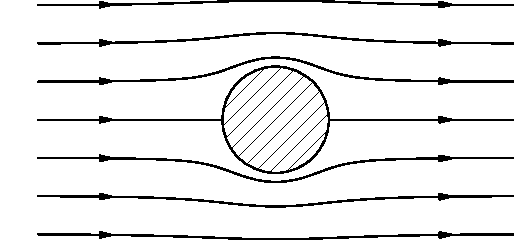
\includegraphics[width=0.35\linewidth]{fyz_fig554a.pdf}}               &
        \subfloat[ ]{\label{fyz_fig554b}
          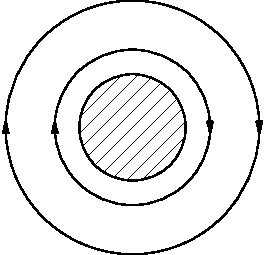
\includegraphics[width=0.15\linewidth]{fyz_fig554b.pdf}}               &
        \subfloat[ ]{\label{fyz_fig554c}
          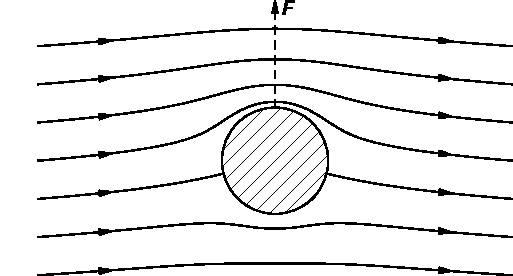
\includegraphics[width=0.35\linewidth]{fyz_fig554c.pdf}}
      \end{tabular}
      \caption{a) Ideální obtékání válce b) Vířivé proudění kolem válce c) Superpozice a) a b)
               (\cite[s.~752]{Feynman02})}
      \label{fyz_fig554}
    \end{figure}
    
    V případě obtékání válce existuje i jiné řešení odpovídající podmínce, že tekutina se ve velké 
    vzdálenosti pohybuje kolem válce po kružnicích. Proudění je pak nové všude jako na obr. 
    \ref{fyz_fig554b}. Takovéto proudění má nenulovou cirkulaci kolem válce, ačkoliv v 
    \emph{tekutině} je \(\symbf{\nabla}\times\bm{v}\) nadále nulové. Jak může existovat cirkulace 
    bez rotace? Cirkulace kolem válce existuje proto, že křivkový integrál \(v\) podél libovolné 
    smyčky, která \emph{obepíná} válec, není nulový. Současně křivkový integrál \(v\) podél 
    uzavřené dráhy, která válec \emph{nezahrnuje}, je nulový. S podobným případem jsme se setkali 
    při výpočtu magnetického pole v okolí vodiče. Rotace \(\bm{B}\) byla mimo vodič nulová, ačkoliv 
    křivkový integrál \(\bm{B}\) podél dráhy, která vodič obklopovala, nulový nebyl. Pole rychlostí 
    při nevířivém proudění kolem válce je přesně totéž jako magnetické pole v okolí vodiče. Pro 
    kruhovou dráhu se středem ve středu válce je křivkový integrál rychlosti
    \begin{equation*}
      \oint\bm{v}\cdot d\bm{s} = 2\pi r v.
    \end{equation*}
    
    V případě nevířivého proudění nesmí integrál záviset na \(r\). Nazvěme jeho konstantní hodnotu
    \(C\); pak platí
    \begin{equation}\label{fyz:eq566}
      v = \dfrac{C}{2\pi r},
    \end{equation}
    kde \(v\) je tangenciální složka rychlosti a \(r\) je vzdálenost od osy válce.
    
    Existuje pěkný způsob demonstrace, jak tekutina cirkuluje kolem otvoru. Vezměme si průhlednou 
    válcovou nádrž s vypouštěcím otvorem uprostřed jejího dna. Naplníme ji vodou, trochu ji 
    roztočíme a vytáhnete zátku z trubice. Uvidíme pěkný jev, znázorněný na obr. \ref{fyz_fig555}. 
    Podobnou věc jste mnohokrát viděli ve vaně!
    
    \begin{figure}[ht!] %\ref{fyz_fig555}
      \centering
      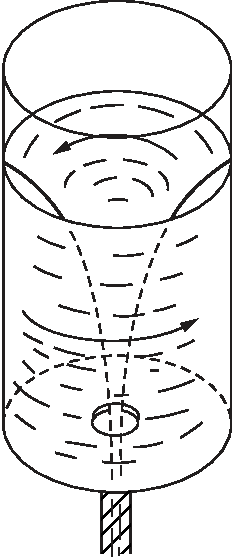
\includegraphics[width=0.3\linewidth]{fyz_fig555.pdf}
      \caption{Voda s cirkulací vytéká z nádrže
               (\cite[s.~752]{Feynman02})}
      \label{fyz_fig555}
    \end{figure}
    
    Ačkoliv jsme na začátku dodali vodě určitou úhlovou rychlost \(\omega\), za chvíli v důsledku 
    viskozity zmizí a proudění se stane nevířivým, ačkoliv kolem otvoru stále existuje určitá 
    cirkulace.
    
    Z teorie umíme vypočítat tvar vnitřní hladiny vody. Jak se částice blíží ke středu, nabývá 
    rychlost. Podle rovnice (\ref{fyz:eq566}) se tangenciální rychlost chová jako \(1/r\). Je to 
    důsledek zachování momentu hybnosti jako v případě krasobruslařky, která přitáhne ruce k tělu. 
    I radiální rychlost se chová jako \(1/r\). Zanedbáme-li tangenciální pohyb, zjistíme, že voda 
    proudí do otvoru radiálním směrem a z rovnice \(\symbf{\nabla}\cdot\bm{v} = 0\) vyplývá, že 
    radiální rychlost je úměrná \(1/r\). Celková rychlost tedy také roste jako \(1/r\) a voda teče 
    podél tzv. \emph{Archimédových spirál}. Hladina mezi vzduchem a vodou je celá pod atmosférickým 
    tlakem a musí tedy mít (na základě rovnice (\ref{fyz:eq560}) následující vlastnost:
    \begin{align*}
      gz + \dfrac{1}{2}mv^2 &= \text{konst}.                                           \\
      \shortintertext{Rychlost \(v\) je však úměrná \(1/r\), takže tvar hladiny je}
      z - z_0               &= - \dfrac{k}{r^2}
    \end{align*}
    
    Zajímavou zvláštností, která se \emph{nevyskytuje v obecném případě} jen v případě nevířivého 
    proudění nestlačitelné tekutiny, je fakt, že známe-li jedno řešení a nějaké jiné řešení, je 
    jejich součet také řešením. Je to pravda, neboť rovnice (\ref{fyz:eq565}) jsou 
    \textbf{lineární}. Úplné rovnice hydrodynamiky (\ref{fyz:eq553}), (\ref{fyz:eq554}) a 
    (\ref{fyz:eq555}) jsou nelineární, a to způsobuje podstatnou odlišnost. V případě nevířivého 
    proudění kolem válce však můžeme složit proudění z obr. \ref{fyz_fig554a} s prouděním z obr. 
    \ref{fyz_fig554b} a získat nové proudové pole na obr. \ref{fyz_fig554c}. Toto proudění je 
    zvláště zajímavé. Rychlost proudění je větší na horním konci válce než na spodním. Tlak na 
    horním konci je tedy nižší než na dolním konci. Máme-li tedy kombinaci cirkulace kolem válce a 
    vodorovného proudění, na válce působí výsledná svislá síla, která se nazývá vztlaková síla. 
    Samozřejmě, není-li cirkulace, podle naší teorie „suché“ vody na žádné těleso žádné výsledné 
    síly nepůsobí.
    
  \section{Vírové čáry}\label{fyz:IIchapXLsecV}
    Už jsme napsali obecné rovnice proudění nestlačitelné tekutiny, pokud v ní existují víry. Jsou 
    tu opět:
    \begin{subequations}\label{fyz:eq567}
      \begin{alignat}{3}
          I&.  \hspace{7em} \symbf{\nabla}\cdot\bm{v}&&=0                    \label{fyz:eq567a} \\
         II&.  \hspace{8em} \symbf{\Omega}     &&=\symbf{\nabla}\times\bm{v} \label{fyz:eq567b} \\
        III&.  \qquad \pder{\symbf{\Omega}}{t}
               \symbf{\nabla}\times(\symbf{\nabla}\times\bm{v}) &&=0         \label{fyz:eq567c}
      \end{alignat}
    \end{subequations}
    
    Helmholtz slovně vysvětlil fyzikální obsah těchto rovnic pomocí tří tvrzení. Nejdříve si 
    představme, že místo proudnic budeme v tekutině kreslit \emph{vírové čáry}. Vírovými čarami 
    chápeme čáry, které mají směr \(\symbf{\Omega}\) a jejich hustota je v libovolné oblasti úměrná 
    velikosti \(\symbf{\Omega}\). Podle rovnice \ref{fyz:eq567b} je divergence \(\symbf{\Omega}\) 
    \emph{vždy} nulová (vzpomeňme si, že podle článku \ref{fyz:IIchapIIIsecVI} je divergence rotace 
    vektoru vždy nulová). Vírové čáry se tedy podobají magnetickým siločarám: nemají začátek ani 
    konec a mají tendenci tvořit uzavřené smyčky. Rovnici \ref{fyz:eq567c} Helmholtz slovně 
    formuloval takto: vírové čáry \emph{se pohybují spolu s tekutinou}. To znamená, že kdybychom 
    označili částice tekutiny pohybující se podél některých vírových čar (mohli bychom je například 
    zbarvit inkoustem), pak by při pohybu tekutiny a přenosu částic tyto částice vyznačovaly nové 
    polohy vírových čar. Nechť se atomy pohybují jakýmkoliv způsobem, vírové čáry se pohybují spolu 
    s nimi. To je jeden způsob vyjádření zákonů hydrodynamiky. 
    
    Naznačuje nám to i jednu metodu řešení libovolných úloh. Je-li dáno počáteční pole proudění 
    (např. hodnoty \(\bm{v}\) ve všech bodech), můžete vypočítat \(\symbf{\Omega}\). Pomocí 
    \(\bm{v}\) můžete také určit, kde se vírové čáry budou nacházet za chvíli; pohybují se 
    rychlostí \(\bm{v}\). Z nového \(\symbf{\Omega}\) můžeme pomocí rovnic \ref{fyz:eq567a} a 
    \ref{fyz:eq567b} určit nové \(\bm{v}\). (Je to stejný problém jako výpočet \(\bm{B}\) z daných 
    proudů.) Známe-li tedy pole proudění v jednom okamžiku, můžeme jej v principu vypočítat pro 
    všechny následující časy. Získáme obecné řešení pro neviskózní proudění. 
    
    \begin{figure}[ht!]
      \centering
      \begin{tabular}{cc}
        \subfloat[ ]{\label{fyz_fig556a}
          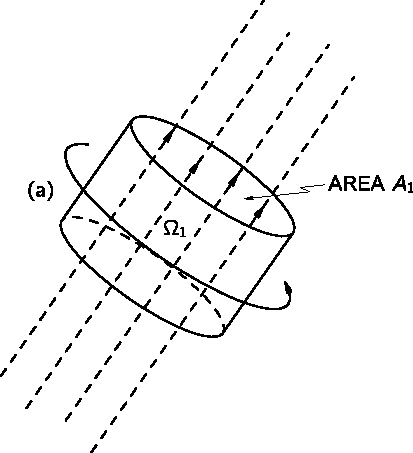
\includegraphics[width=0.4\linewidth]{fyz_fig556a.pdf}}               &
        \subfloat[ ]{\label{fyz_fig556b}
          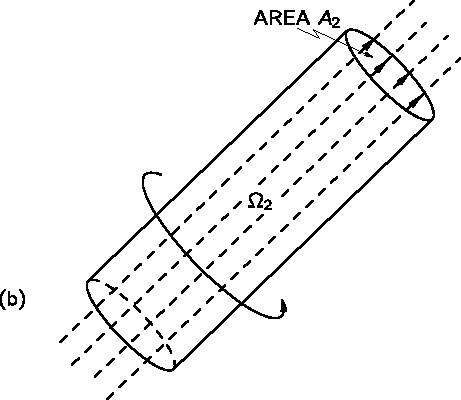
\includegraphics[width=0.4\linewidth]{fyz_fig556b.pdf}}              
      \end{tabular}
      \caption{a) Skupina vírových čar v čase \(t\). b) Tytéž čáry v čase \(t'\).
               (\cite[s.~755]{Feynman02})}
    \end{figure}

    Dále bychom chtěli ukázat, jak lze alespoň z části pochopit Helmholtzovo tvrzení, a tedy i 
    rovnici \ref{fyz:eq567c}. Ve skutečnosti je to jen zachování momentu hybnosti, použité v 
    případě tekutiny. Představme si malý váleček v kapalině, jehož osa je rovnoběžná s vírovými 
    čarami (obr. \ref{fyz_fig556a}). O něco později se \emph{tatáž} část tekutiny bude nacházet 
    někde jinde. 
    
    Obecně bude mít tvar válce s jiným průměrem a na jiném místě. Může mít i jinou orientaci (jako 
    na obr. \ref{fyz_fig556b}). Pokud se však průměr změnil, výška válce se musela 
    zvětšit, aby objem zůstal konstantní (neboť předpokládáme nestlačitelnost tekutiny). Jelikož 
    jsou kromě toho vírové čáry vázány na danou látku, jejich hustota se zvýší, když se průřez 
    válce zmenší. Součin velikosti vírového vektoru \(\symbf{\Omega}\) a plochy \(\bm{S}\) průřezu 
    válce bude konstantní, takže podle Helmholtze musí platit
    \begin{equation}\label{fyz:eq568}
      \Omega_1S_1 = \Omega_2S_2
    \end{equation}
    
    Nyní si všimněme, že při nulové viskozitě jsou všechny síly na povrchu válce (nebo vlastně 
    \emph{libovolného} objemu) kolmé na povrch. Tlakové síly mohou způsobit přemístění daného 
    objemu z jednoho místa na jiné, nebo jej donutit změnit tvar; nepůsobí-li však 
    \emph{tangenciální} síly, nemůže se velikost \emph{momentu hybnosti látky} v daném objemu 
    změnit. Moment hybnosti tekutiny ve válečku je roven součinu jeho momentu setrvačnosti \(I\) a 
    úhlové rychlosti tekutiny, která je úměrná vírnatosti \(\symbf{\Omega}\). V případě válce je 
    moment setrvačnosti úměrný \(mr^2\). Na základě zachování momentu hybnosti tak docházíme k 
    závěru, že
    \begin{equation*}
      (m_1r_1^2)\Omega_1 = (m_2r_2^2)\Omega_2.
    \end{equation*}
    Hmotnost je však stejná, \(m_1 = m_2\), a průřezy jsou úměrné \(r^2\), takže zde máme opět 
    vztah (\ref{fyz:eq568}). Helmoltzovo tvrzení, které je ekvivalentní s rovnicí \ref{fyz:eq567c}, 
    je jen důsledkem skutečnosti, že bez viskozity se moment hybnosti elementu tekutiny nemůže 
    změnit.
    
    \begin{figure}[ht!] %\ref{fyz_fig557}
      \centering
      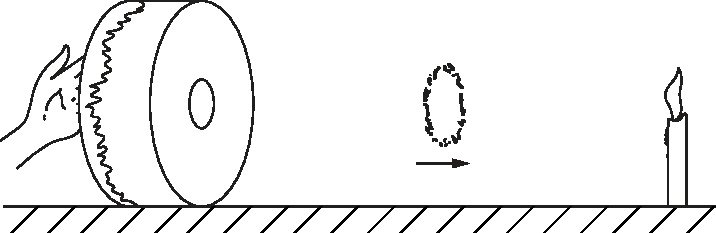
\includegraphics[width=0.7\linewidth]{fyz_fig557.pdf}
      \caption{Jak vytvořit putující vírový prstenec
               (\cite[s.~755]{Feynman02})}
      \label{fyz_fig557}
    \end{figure}
    
    Pohybující se vír lze pěkně demonstrovat pomocí jednoduchého zařízení na obr. \ref{fyz_fig557}. 
    Je to „buben“ s průměrem a délkou asi \SI{60}{cm}, který získáme, napneme-li silnou gumovou 
    fólii na otevřený konec válcové „krabice“. Buben je překlopen na stranu a jeho dno je pevné s 
    výjimkou otvoru, který má průměr asi \SI{8}{cm}. Udeříme-li prudce na gumovou membránu, vyrazí 
    z otvoru vírový prstenec.
    
    Ačkoliv je neviditelný, můžeme se o jeho existenci přesvědčit podle toho, že sfoukne plamen 
    svíčky ve vzdálenosti \num{3}-\SI{6}{m}. Ze zpoždění tohoto jevu poznáme, že „něco“ se šíří 
    prostorem konečnou rychlostí. Lépe to uvidíme, nafoukáme-li nejdříve do krabice trochu dýmu. 
    Pak uvidíme vír jako krásný okrouhlý prstenec.
    
    Dýmový prstenec je vlastně prstencový svazek vírových čar (obr. \ref{fyz_fig558a}). Jelikož 
    \(\symbf{\Omega} = \symbf{\nabla}\times\bm{v}\), popisují vírové čáry zároveň cirkulaci vektoru 
    \(\bm{v}\) jak ukazuje na obrázku \ref{fyz_fig558b}. To, proč se prstenec pohybuje dopředu, 
    můžeme pochopit následujícím způsobem: cirkulující rychlost ve spodní části prstence se šíří k 
    jeho horní části a má tak složku rychlosti ve směru osy. Jelikož se vírové čáry pohybují spolu 
    s tekutinou, i ony se pohybují vpřed rychlostí \(\bm{v}\). (Samozřejmě, že cirkulace rychlosti 
    \(\bm{v}\) horní části zajišťuje i dopředný pohyb vírových čar ve spodní části.)
    
    \begin{figure}[ht!]
      \centering
      \begin{tabular}{cc}
        \subfloat[ ]{\label{fyz_fig558a}
          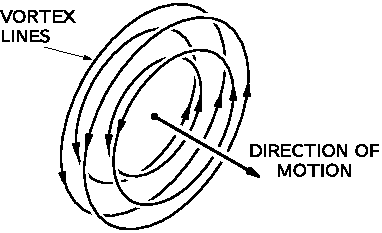
\includegraphics[width=0.5\linewidth]{fyz_fig558a.pdf}}               &
        \subfloat[ ]{\label{fyz_fig558b}
          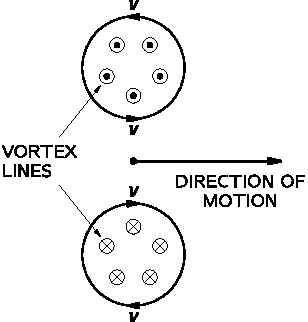
\includegraphics[width=0.4\linewidth]{fyz_fig558b.pdf}}              
      \end{tabular}
      \caption{Pohybující se vírový (dýmový) prstenec. a) Vírové čáry. b) Průřez prstence.
               (\cite[s.~756]{Feynman02})}
    \end{figure}
    
    Musíme se zmínit ještě o jedné vážné komplikaci. Už jsme poznamenali, že z rovnice 
    (\ref{fyz:eq554}) vyplývá, že je-li \(\symbf{\Omega}\) na počátku nulové, bude nulové vždy. 
    Tento výsledek znamená neúspěch teorie „suché“ vody, neboť znamená, že když je 
    \(\symbf{\Omega}\) nulové jednou, bude takové vždy - žádným způsobem není možné vyrobit víry. V 
    našem jednoduchém pokusu s bubnem jsme však vytvořili vírový prstenec ve vzduchu, který byl 
    původně nehybný. (Před úderem bylo zaručeně všude v krabici \(\bm{v} = 0\) a 
    \(\symbf{\Omega}=0\).) Také víme, že na jezeře můžeme vytvořit víry pomocí pádla. Je zřejmé, že 
    k tomu abychom úplně pochopili chování tekutin, musíme přejít k teorii „mokré“ vody.
    
    Další tvrzení teorie „suché“ vody, které není správné, je obsaženo v předpokladu, který jsme 
    provedli, když jsme uvažovali o proudění tekutiny na hranici s pevnou látkou. Když jsme 
    hovořili o obtékání válce (jako např. na obr. \ref{fyz_fig554}), předpokládali jsme, že 
    tekutina sklouzne po povrchu pevné látky. V naší teorii by rychlost na povrchu pevné látky 
    mohla mít libovolnou hodnotu v závislosti na počátečních podmínkách; neuvažovali jsme „tření“ 
    mezi tekutinou a pevnou látkou. Je však experimentálním faktem, že rychlost skutečné tekutiny 
    vždy klesá u povrchu pevného tělesa k nule. Naše řešení pro případ válce (ať už s cirkulací, 
    nebo bez ní) je proto chybné podobně jako náš výsledek, který se týká vzniku vírů. O 
    správnějších teoriích si povíme v následující kapitole.
    
  \section{Příklady a cvičení}\label{fyz:IIchapXLsecVI}
  

  
} %tikzset
%---------------------------------------------------------------------------------------------------
\printbibliography[title={Seznam literatury},heading=subbibliography]
\addcontentsline{toc}{section}{Seznam literatury}